\chapter{Odometry Module}
\label{cha:vodom}
Visual odometry is the process of determining the position and
orientation (the pose) of a camera relative to a given target by
analyzing a sequence of images. Contrarily to object tracking in
image coordinates, visual odometry needs calibrated cameras. It 
implies the knowledge of camera intrinsic parameters. Consequently, 
the \lstinline$Rox_Camera$ object shall be fed with the correct 
camera  intrinsic parameters. Incorrect camera intrinsic parameters
will produce an incorrect localization.

The localization of the camera in the environment can be useful in several applications such as robotics, augmented reality, and many others.\\

The Odometry module contains the following sub-modules:

\begin{description}
% \item[Odometry Parameters]~: module with structures and methods for handling the tracking parameters
  \item[Odometry Single Plane]~: module with structures and methods for camera localization relative to a single plane
  \item[Odometry Multi Planes]~: module with structures and methods for camera localization relative to a multi planes
  \item[Odometry Inertial Observer]~: module with structures and methods for camera localization with inertial observer
\end{description}

\section{Visual odometry observing a single plane}
\label{sec:vodm_single_plane}

\subsection{Odometry parameters}
\label{sse:odometry_single_plane_params}

\subsubsection{The {\tt Rox\_Odometry\_Params} object}
\label{sss:odometry_single_plane_params_object}

A \lstinline$Rox_Odometry_Single_Plane_Params$ object can be defined using the pointer to a \lstinline$Rox_Tracking_Params_Structure$:
\begin{lstlisting}
typedef struct Rox_Tracking_Params_Struct* Rox_Odometry_Single_Plane_Params;
\end{lstlisting}
The structure is opaque to the users.

\subsubsection{Creating/Deleting a {\tt Rox\_Odometry\_Params}}
\label{sss:odometry_single_plane_params_newdel}

Functions are provided to allocate and deallocate a \lstinline$Rox_Odometry_Single_Plane_Params$ object~:

\begin{lstlisting}
Rox_Error rox_odometry_single_plane_params_new (Rox_Odometry_Single_Plane_Params *params);
\end{lstlisting}
The \lstinline$rox_odometry_single_plane_params_new$ function allocates memory for the odometry object and returns a pointer on the newly created object.

\begin{lstlisting}
Rox_Error rox_odometry_single_plane_params_del (Rox_Odometry_Single_Plane_Params *params);
\end{lstlisting}
The function deallocates memory for a \lstinline$Rox_Odometry_Single_Plane_Params$ object. It is necessary to call this function when the object is not used anymore. \\

\subsubsection{Main functions related to {\tt Rox\_Odometry\_Params}}
\label{sss:odometry_single_plane_params_methods}

% \paragraph{Localization relative to objects with known size}
% \label{par:odometry_model}
% ~\\~\\
The camera localization is done relative to a known object. It is
assumed that a rectangular planar object with size (sizx, sizy) is
observed. In this case it is possible to know the pose of the camera
relative to the planar object (the object frame is centered on the
rectangular object, see figure~\ref{model_size}) and also the
displacement of the camera between two images.

\begin{figure}[htbp] 
\begin{center}
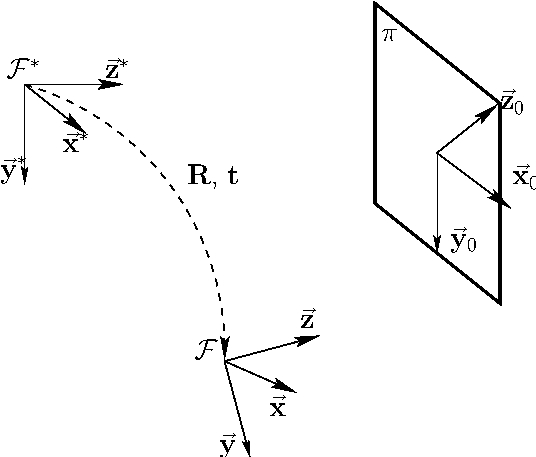
\includegraphics[width=0.75\textwidth]{odometry/figures/model_size}
\caption{Localization relative to a planar object with known size.}
\label{model_size}
\end{center}
\end{figure}

% \paragraph{Localization relative to objects with known normal}
% \label{par:odometry_scale}
% ~\\~\\
% If the camera localization is done relative to a known object the user shall set the scaled normal of the plane using the following function:

% \begin{lstlisting}
% Rox_Void rox_odometry_single_plane_params_set_model_normal(Rox_Odometry_Single_Plane_Params P, Rox_Vector nd)
% \end{lstlisting}

% \begin{figure}[htbp] 
% \begin{center}
% 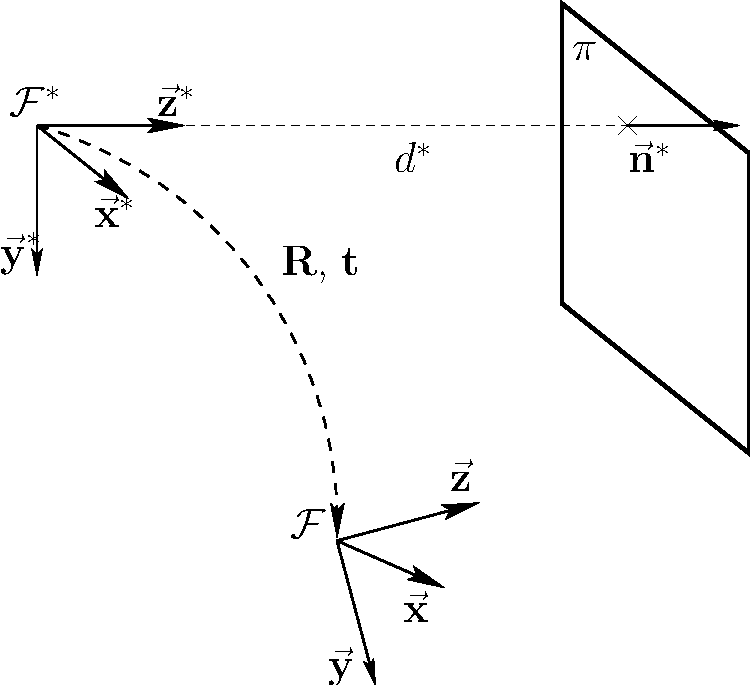
\includegraphics[width=0.5\textwidth]{odometry/figures/model_norm}
% \caption{Localization relative to a planar object with unknown size.}
% \label{model_norm}
% \end{center}
% \end{figure}



\subsection{Visual odometry Single Plane}
\label{sse:odometry_single_plane}

\subsubsection{The {\tt Rox\_Odometry\_Single\_Plane} object}
\label{sss:odometry_single_plane_object}

A \lstinline$Rox_Odometry_Single_Plane$ is a pointer to the opaque structure \lstinline$Rox_Odometry_Single_Plane_Structure$:
\begin{lstlisting}
typedef struct Rox_Odometry_Single_Plane_Struct *Rox_Odometry_Single_Plane;
\end{lstlisting}

\subsubsection{Creating/Deleting a {\tt Rox\_Odometry\_Single\_Plane}}
\label{sss:odometry_single_plane_newdel}
Functions are provided to allocate and deallocate a \lstinline$Rox_Odometry_Single_Plane$ object~:

\begin{lstlisting}
Rox_Error rox_odometry_single_plane_new (Rox_Odometry_Single_Plane *odometry, Rox_Odometry_Single_Plane_Params params, Rox_Model_Single_Plane model);
\end{lstlisting}
The function allocates memory for the odometry object, according to
the 'model' and `params' parameters and returns a pointer on the newly created object.

\begin{lstlisting}
Rox_Error rox_odometry_single_plane_del (Rox_Odometry_Single_Plane *odometry);
\end{lstlisting}
The function deallocates memory for a \lstinline$Rox_Odometry_Single_Plane$ object. 
It is necessary to call this function when the object is not used anymore. \\

\subsubsection{Main functions related to {\tt Rox\_Odometry\_Single\_Plane}}
\label{sss:odometry_single_plane_methods}
The main functions to manipulate a \lstinline$Rox_Odometry$ object are~:
\begin{description}
  \item[rox\_odometry\_single\_plane\_make]: Performs the visual odometry when the
  displacement of the target is not too large~;
  \item[rox\_odometry\_single\_plane\_get\_pose]: Returns the pose matrix~;
  \item[rox\_odometry\_single\_plane\_set\_pose]: Set the pose matrix~;
  \item[rox\_odometry\_single\_plane\_get\_score]: Returns the quality score of visual odometry~;
\end{description}

Please refer to the Programmer Manual for further information about visual odometry functions, 

\subsubsection{Target identification}
\label{sss:odometry_single_plane_dent}
~\\~\\
When the displacement of the target is very large in the image, it is sometimes necessary to search the target in the whole image. The same problem can arise when the target is lost, occluded or out of the image and comes back in the camera field of view. \rox{} allows the user to identify the target by choosing several identification methods. The methods are detailed in section~\ref{sec:ident}. See the example ``rox\_example\_odometry\_single\_plane.c'' for odometry with identification using a textured image and ``rox\_example\_odometry\_single\_plane\_database.c'' for odometry with identification using a database of textured images.

If the user needs a very robust identification we recommend to use a
photoframe around the target. Section \ref{sse:ident_photoframe}
describes how to build photoframes and use them for target
identification.  See the example ``rox\_example\_odometry\_single\_plane\_photoframe.c'' for an
example of use with the odometry.

% \input{odometry/rox_example_odometry.tex}
% \input{odometry/rox_example_odometry_photoframe.tex}


\section{Visual odometry observing multi planes}
\label{sec:vodm_multi_plane}

%\input{odometry/odometry_m3d_params.tex}

\subsection{Visual Odometry Multi Plane}
\label{sse:odometry_multi_plane}

The odometry module enables tracking of a textured convex polyhedron of $n$ faces whose real
dimensions are known. The estimation of the camera pose is obtained whatever the part of the object the 
camera is looking at. The object is considered as a whole and the module uses all visible information 
to get a precise and stable localization of the object. The simplest example of a convex polyhedron 
is a cube (6 faces). The object to track using this module shall be textured on all the faces. Constraints
related to texture are similar to those of 2D planar odometry. 

\subsubsection{The {\tt Rox\_Odometry\_Multi\_Plane} object}
\label{sss:odometry_multi_plane_object}

A \lstinline$Rox_Odometry_Multi_Plane$ object is a pointer to the \lstinline$Rox_Odometry_Multi_Plane_Struct$ structure:
\begin{lstlisting}
typedef struct Rox_Odometry_Multi_Plane_Struct* Rox_Odometry_Multi_Plane;
\end{lstlisting}
The structure is opaque to the users.

\subsubsection{Creating/Deleting a {\tt Rox\_Odometry\_Multi\_Plane}}
\label{sss:odometry_multi_plane_newdel}
Functions are provided to allocate and deallocate a \lstinline$Rox_Odometry_Multi_Plane$ object~:

\begin{lstlisting}
Rox_Odometry_Multi_Plane rox_odometry_multi_plane_new(Rox_Odometry_Multi_Plane_Params params, Rox_Model_Multi_plane model);
\end{lstlisting}
The function allocates memory for the odometry object, according to the {\tt model} and {\tt params} parameters and returns a pointer on the newly created object.

A 3D object model shall be passed to the odometry module for an appropriate odometry process (see section~\ref{sec:model_multi_plane}). 
The precision of the 3D vertices passed as input is the key to the accuracy of the odometry results. 3D vertices are used 
to simulate the object image projection. If the vertices are not well defined, the alignment of the real object and the virtual 
object is not possible. Scale of the vertices is not important for the visual odometry. However the output pose varies with 
the input scale.

Carefully choosing textures is very important for a robust odometry. The picture captured for each quadrilateral shall be as much 
parallel as possible relative to the face. Blur, noise and other lighting artefacts shall be avoided. Textures shall be as big as 
possible (e.g. a 512{*}512 texture per quadrilateral). If possible, use the same device for capturing the texture and for the 
odometry process, in order to minimize differences between images.

\begin{lstlisting}
Rox_Void rox_odometry_multi_plane_del(Rox_Odometry_Multi_Plane odometry);
\end{lstlisting}
The \lstinline$rox_odometry_multi_plane_del$ function deallocates memory for a \lstinline$Rox_Odometry_Multi_Plane$ object. It is necessary to call this function when the object is not used anymore. \\

\subsubsection{Main functions related to {\tt Rox\_Odometry\_Multi\_Plane}}
\label{sss:odometry_multi_plane_methods}

The main functions to manipulate a \lstinline$Rox_Odometry_Multi_Plane$ object are~:
\begin{description}
  \item[rox\_odometry\_multi\_plane\_make]: Performs the visual odometry and update the camera pose~;
  \item[rox\_odometry\_multi\_plane\_get\_pose]: Returns the pose matrix~;
  \item[rox\_odometry\_multi\_plane\_set\_pose]: Set the pose matrix~;
  % \item[rox\_odometry\_get\_score]: Returns the quality score of visual odometry~;
\end{description}

Please refer to the Programmer Manual for further information about visual odometry functions.
See the example ``rox\_example\_odometry\_multi\_plane.c'' for an example of use.


\section{Visual odometry with an inertial observer}

\subsection{Visual and Inertial Odometry}
\label{sse:odometry_visual_inertial}

When the displacement between two successive images is too large, the visual odometry may fail. Consequently, it is necessary to identify the target to get the camera pose relative to the known model. Using an inertial sensor allows us to get a high rate prediction of the target position in the image even if the displacement is very important. The visual odometry may be successful as long as the inertial prediction is precise enough. As the inertial prediction does not depend on the actual scene viewed by the camera, it is possible to predict the target position even if it is out of the camera field of view. Consequently, when the target reappears in the camera field of view, no identification method will be necessary to make visual odometry if the inertial prediction is close enough from the real target position. \\
Note that to make an efficient visual - inertial odometry, the calibration pose between the two sensors shall be known by the user and the target frame shall coincide with the local tangent plane used as reference for the inertial measures.    

\subsubsection{Main functions related to {\tt Rox\_Odometry\_Visual\_Inertial}}
\label{sss:odometry_visual_inertial_methods}

The main functions to manipulate visual - inertial odometry are~:
\begin{description}
  \item[rox\_odometry\_visual\_inertial\_init\_async\_observer]: Performs the detection of the given target and initializes the inertial observer using the odometry results. This function initializes an asynchronous observer implying that visual and inertial data have to be precisely dated. The dating shall be expressed in seconds and have the same time reference for both inertial and visual data (i.e using the UTC time)~;
  \item[rox\_odometry\_visual\_inertial\_init\_sync\_observer]: Performs the detection of the given target and initializes the inertial observer using the odometry results. This function initializes a synchronous observer~;
  \item[rox\_odometry\_visual\_inertial\_make]: Makes the visual - inertial odometry. Note that the inertial observer can be reinitialized by a visual detection method if the target has been lost during 10 successive images~;
  \item[rox\_odometry\_visual\_inertial\_get\_matsl3\_prediction\_copy]: Gets a copy of the initialization homography~;
\end{description}

If you need further information about visual and inertial odometry functions, please refer to the Programmer Manual.
See the example ``rox\_example\_odometry\_visual\_inertial.tex'' for an
example of use.

% \input{odometry/rox_example_odometry_visual_inertial.tex}

